\chapter{Brain circuitry (Neuronal connectivity)}
\label{chap:brain_circuitry}

Essentially, the nerve cell A receives the summated signal from the many
dendritic spines (Sect.\ref{sec:dendritic_spines}) at the postsynaptic side of
the synapse. Once the signals reach the action potential initiation site, i.e.
axon hillock (Sect.\ref{sec:axon-hillock}), and pass a threshold, an neuronal
spike is activated and the electrical signal propagates along the axon before
reaching the presynaptic side of the synapses formed by the axons of neuron A
with the other neurons. The details of this mechanism is explained in
Sect.\ref{sec:neuron_connectivities}.

The first and widely studies in neuroscience are from the frog neuromuscular
junction (to study mechanism of synaptic transmission -
Sect.\ref{sec:synaptic_transmission}) and squid giant synapse, which was first
reported by Young \cite{young1936}.

The axon may have myelin sheaths.
\begin{itemize}
  \item the neural pathway with myelinated axons appear as bright white
  \item the neural pathway with unmyelinated axons appear as darker beige color
\end{itemize}

The complexity of the brains not only comes from the diversed
electrical properties of the different neuron types; but also in the
connectivity among them, within a region and across regions.

From breathing to thinking and even reading a book, our neurons are triggered
and fired and are literally re-wired, building millions of new connections a
second. Every second, the neuro-circuitry of our brain is modified, making us
truly a different person every second we live.
This adaptability, both conscious and unconscious, is often termed {\bf
neural plasticity} whose basic mechanism at
the cellular level is synaptic plasticity (Sect.\ref{sec:synaptic_plasticity}).

Along with the strengthen or weaken of synaptic strength, the formation and
death of a synapse is also important (Sect.\ref{sec:synaptogenesis}).
The formation of proper axonal branches is a critical step in the
establishment of functional neural circuits (Sect.\ref{sec:Axon}).

Our understanding of the neuronal connectivity mainly comes from mice (white
mouse). The choice of mouse for histology due to 2 things
\begin{enumerate}
  \item abundant (as staining is still largely a question of luck -
  Sect.\ref{sec:stain-neuron}).
  
  \item small brain (whenever serial seciton of the whole brain is required)
  
  \item lyssencephalic layout of the cortex, i.e. almost complete absence of
  folds
  
  \item more homogeneous build of mouse cortex compared to the variety of
  cortical areas in human brain.
  
Rodents' brains are also used (lesser variety of neuronal morphology)
\end{enumerate}
Sect.\ref{sec:stain-neuron} describes different experimental techniques to
'visualize' the neurons.

% ``Re-wire'' can be achieved by adjusting the connection strength, known as {\bf
% synaptic plasticity} and the rate of firing signaling.
% This is postulated in the {\bf dynamic link architecture} (DLA) hypothesis
% (Sect.\ref{sec:DLA_hypothesis}.


\begin{figure}[htb]
  \centerline{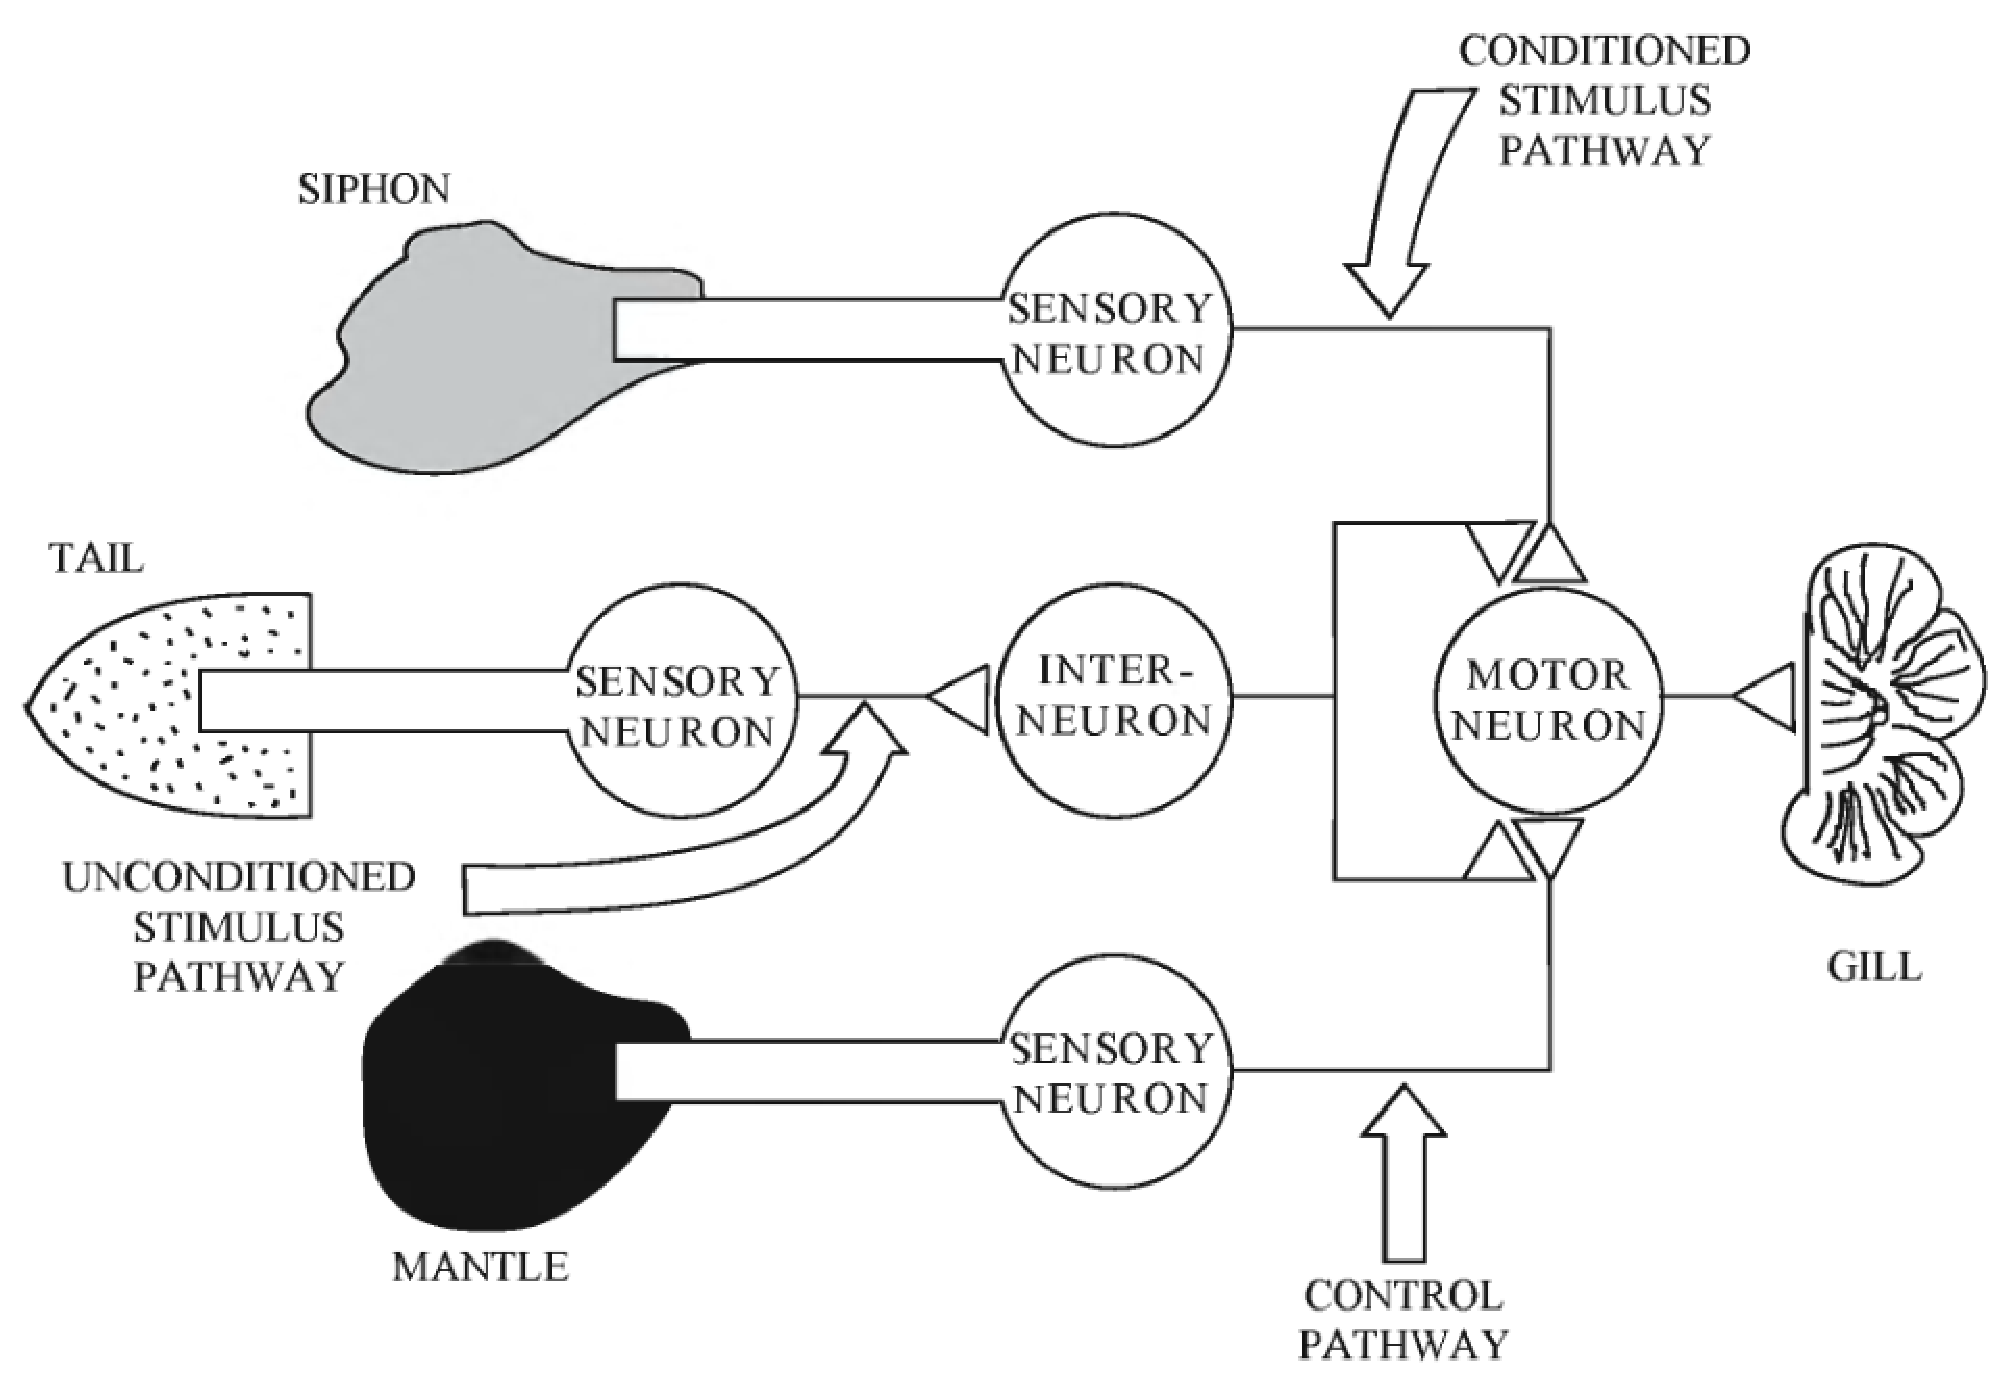
\includegraphics[height=6cm]{./images/parallel_neurons.eps}}
  \caption{Schematic diagram of neural circuitry of sea hare with
    various types of response}\label{fig:neural_circuitry_sea-hare}
\end{figure}

Example: knee-jerk
or stretch reflex \url{http://nba.uth.tmc.edu/neuroscience/m/s1/chapter06.html}



\section{Neural pathways}

All cells possess transmembrane signaling systems
that allow them to receive information from extracellular
stimuli like hormones, neurotransmitters, or sensory
stimuli. This fundamental process allows cells to communicate
with each other.

All transmembrane signaling systems share two basic elements, a receptor which
is able to recognize an extracellular stimulus as well as an effector which is
controlled by the receptor and which can generate an intracellular signal.

Once the functional purpose of different brain structures have been found,
the neural pathways are named by their origin and termination.
\begin{itemize}
  \item nigrostriatal pathway: this pathway runs from the {\it subtantia nigra}
  (Sect.\ref{sec:substantia_nigra}) to the corpus striatum (Sect.\ref{sec:striatum})
  
  \item cerebellorubrothalamocortical pathway: this pathway originates from
  cerebellum, synapses in the red nucleus (Sect.\ref{sec:nuclei_structure}), on
  to the thalamus (Sect.\ref{sec:thalamus}) and finally terminating in the
  cerebral cortex (Sect.\ref{sec:cerebral_cortex})
\end{itemize}

\url{http://en.wikipedia.org/wiki/Neural_pathway}


\section{Brain circuits}

\subsection{Papez circuit}
\label{sec:Papez_circuit}

The {\bf Papez circuit} (or medial limbic circuit), is a neural circuit
suggested by James Papez (1973) that was believed to control of emotional
expression. Even though this circuit is not completely accurate, it serves
as an important ground for the next discoveries.

Paul D. MacLean reconceptualized Papez's proposal and coined the term limbic
system. In the modified version of the circuit, amygdala was added as it is
thought to play a key role in emotion, a structure that was not a part of the
Papez circuit (Sect.\ref{sec:limbic-system}.

Here is the original Papez's neural circuit:
\begin{verbatim}
the hippocampal formation and the cingulate gyrus constitutes the neural
substrate of emotional behavior
\end{verbatim}
Sect.\ref{sec:hippocampal_formation}, Sect.\ref{sec:cingulate_gyrus}.
%the circuitry start and end with the hippocampus)

The pathway:  hippocampal formation $\rightarrow$ fornix $\rightarrow$
mammillary bodies $\rightarrow$ mammillothalamic tract
$\rightarrow$ anterior thalamic nucleus $\rightarrow$ cingulum
$\rightarrow$ entorhinal cortex (EC) $\rightarrow$ hippocampal formation.




\subsection{Yakovlev circuit}
\label{sec:Yakovlev-circuit}

\url{http://www.ncbi.nlm.nih.gov/pubmed/17511282}

\section{Basal ganglia macrocircuits}
\label{sec:basal-ganglia-macrocircuit}

The components of basal ganglia is discussed in Sect.\ref{sec:basal-ganglia}.

The basal ganglia macrocricuit described here is based on the Rate Model -
Sect.\ref{sec:RateModel-BG} in that the cortico-basal ganglia loops are composed
of several parallel, segregated, and functionally distinct, but homologous
closed-loops - Sect.\ref{sec:basal-ganglia-parallel-closed-loop}. 

For each loop, basal ganglia (BG) macrocircuit; comprising the
neostriatum (caudate/putamen and nucleus accumbens), the Globus Pallidus
(internal and external), the substantia nigra (pars reticulata and compacta),
and the subthalamic nucleus (STN), are a highly interconnected set of
subcortical nuclei.

\subsection{parallel closed-loop}
\label{sec:basal-ganglia-parallel-closed-loop}


\begin{mdframed}
Despite their parallel organization (as we are going to discussed below), the
cortico-basal ganglia loops should be viewed more as a continuum rather than
subdivisions with strict boundaries - Sect.\ref{sec:split-loop}).

\end{mdframed}

There are five parallel and largely (somato-topically organized) segregated
circuits: motor, oculomotor, dorsolateral prefrontal, lateral orbitofrontal and
limbic.
\begin{enumerate}
  \item motor loop (voluntary movement): Sect.\ref{sec:motor-loop-voluntary-movement}
  
  \item oculomotor loop - Sect.\ref{sec:oculomotor-loop}
\end{enumerate}
The names reflect the major cortical area(s) of origin and function of each.
Major hypothesis: information flows from the cortex, through the striatum,
pallidum and thalamus, before returning to the major cortical area from which
each circuit originated. So, the cortical input areas are also the cortical
output areas from which each circuit originated. This forms the {\bf
closed-loop}.

Thus, injury to a particular circuit would result in selective disturbances in
motor, cognitive or emotional behavior. Potentially, this scenario allows little
if any interloop communication.

\subsection{split-loop}
\label{sec:split-loop}
\label{sec:split-loop-model}

In the traditional cortico-striato-thalamo-cortical connections with 5 parallel,
and segregated pathways, i.e. no interactions between any two pathways
(Sect.\ref{sec:parallel-pathways}). However, recent anatomic, functional, and
clinical data suggests there exists a cross-communication between circuits (the
GPe (Sect.\ref{sec:GPe}) relay appearing critical for this); meaning that a
particular striatal area (via its open loop, can influence a cortical field it does not project to,
allowing for the theoretical coexistence of different symptoms in response to a
[functional] lesion in only one of the affected circuits.

The projections from the MI, SMA, and PM partially overlap in the striatum.
Because of that, the refinement to closed-loop model is the {\bf split-loop}
model which allows for cross-communication between circuits (the GPe relay
appearing critical for this); meaning that a particular striatal area (via its
open loop, can influence a cortical field it does not project to, allowing for
the theoretical coexistence of different symptoms in response to a [functional]
lesion in only one of the affected circuits. This may be especially pertinent to
HD, where selected atrophy of cortical and BG subregions may be an indicator of
symptom presentation.

\section{Cortico-cortical circuit}
\label{sec:cortico-cortical-projection}
%Neurons connection in cortex: 

The cortex is anatomically divided into different layers
(Sect.\ref{sec:layered_structure}).

In barrel cortex of adult mice in response to whisker stimulation:
Sensory input from the whisker pad is received by neurons in cortical layer 4
through the sensory signaling pathway.

The excitatory input from layer 4 to layer 2/3 neurons is strictly feedforward
and makes glutamatergic synapses onto layer 2/3 neurons.

\section{Cx-STN-GPi/SNr circuit (hyperdirect pathway)}
\label{sec:hyperdirect-pathway}

The cortex also project directly to the subthalamic nucleus which is the
hyperdirect pathway to the control of BG output.

\section{Cortico-striatal circuit}
\label{sec:cortico-striatal-projection}
\label{sec:cortico-striatal-loops}

Cortex provides one of the major excitatory inputs to the striatum, which was
first described by Webster in the 1960s in rat and cat \citep{webster1961,
webster1965}; and studies on rabbit and money by other groups.
The common conclusion was that all major cortical areas project to the striatum,
though the visual cortices targeted rather restricted striatal areas compared to
other cortical regions (Sect.\ref{sec:visual-cortex}).

The first model of cortio-striatal connections was proposed by Kemp and Powell
(1970). \footnote{\url{http://en.wikipedia.org/wiki/Caudate_nucleus}}

Cortical neurons projecting to the striatum outnumber striatal medium spiny
neurons by about a factor of 10 (Zheng and Wilson, 2002).

MSN in two structurally similar but neurochemically distinct compartments in the
striatum: striosomes and matrix; receives different cortical inputs.  
\begin{enumerate}
  
  \item MSN in striosomes (striosomal MSN): receiving   convergent   limbic   and   prelimbic inputs   

  \item MSN in matrix: receiving convergent  input  from  ipsilateral  primary
  motor  and sensory motor cortices and contralateral primary motor cortices
  (Leckman, 2002; Mink, 2006)
  
\end{enumerate}

\subsection{input to MSN}

In addition to the cortical input, MSN also receive other inputs, so that its
spiking activity is partly dependent on {\it perceptual cues} that are judged
salient, so rewarding (e.g. Dopamine) and aversive stimuli (e.g. GABAergic input from
???) can both serve as cues (Canales and Graybiel, 2000).
Specifically,  they  are
responsive to dopaminergic inputs from the substantia
nigra,  and  these  signals  probably  participate  in  the
calculation  of  perceived  salience  (reward  value)  of
perceptual  cues  along  with  excitatory   inputs  from
midlinethalamicnucle


GABAergic inputs:
\begin{enumerate}
  \item  other less abundant striatal cell types (probably in modulating habit
  learning):

\begin{itemize}
  \item  cholinergic tonically active neurons (TANs)

 \item   and fast-spiking GABAergic interneurons (Gonzalez-Burgos et al., 2005;
 Jog et al., 1999)
  
\end{itemize}


\end{enumerate}

\subsection{input to FSN}

The fast-spiking spiny interneurons (Sect.\ref{sec:fast-spiking-interneuron}) of
the striatum receive direct cortical inputs predominantly from lateral cortical 
regions,  including  the  primary  motor  and somatosensory cortex, and they are
highly sensitive to cortical activity in these regions. They are also known to
be  electrically  coupled  via  gap  junctions  that  connect adjacent 
dendrites.

Once  activated,  these  fast-spiking neurons  can  inhibit  many  nearby 
striatal  projection neurons synchronously via synapses on cell bodies and
proximal dendrites (Koos and Tepper, 1999).

\section{Cortico-striato-thalamo-cortical pathway}
\label{sec:cortico-striato-thalamo-cortical-pathway}
\label{sec:parallel-pathways}

{\bf Cortico-striato-thalamo-cortical connections/pathways} refers to the
{\bf closed-loop} circuit of information traversial via the basal ganglia, i.e.
information flows from the cortex, through the striatum, pallidum and thalamus,
before returning to the major cortical area from which each circuit originated.
Thus the cortical input areas are also the cortical output areas from which each
circuit originated.

In Rate Model (Sect.\ref{sec:RateModel-BG}), cortico-striatao-thalamo-cortical
connections have 5 {\bf parallel pathways} (if refes to the source); each
associated with the major cortical area(s) of origin and function of each.
\begin{enumerate}
  \item motor, 
  
  \item oculomotor, Sect.\ref{sec:ocular-dominance-column}
  
  \item dorsolateral prefrontal, 
  
  \item lateral orbitofrontal and

  \item limbic
\end{enumerate}
These are often 'collapsed' functionally into distinctions of motor, associative
and limbic circuits. This implies the agreed hypothesis that (1) they are
segreated closed loop; and (2) injury to a particular circuit would result in
selective disturbances in motor, cognitive or emotional behavior. 
However, remember that this is not always agreed, as 
there are recent evidences of local connectivity (i.e. cross-communication) as
you should read 'split-loop' model - Sect.\ref{sec:split-loop-model}.

There are two major brain structures involving in motor control:
cerebellum and basal ganglia.

\begin{itemize}
  \item The cerebellum (Sect.\ref{sec:cerebellum}) receives the sensory info through the 
spinocerebellar tract (Sect.\ref{sec:spinal_cord}).

  \item The basal ganglia gets it from the cortex, hence "cortico-striato" (from
  the word striatum which is part of the basal ganglia).   
\end{itemize}
Thus it is called {\bf cortio-striato}.

A motor plan starts in the cortex, is then sent to the basal ganglia(in this
example the striatum), then it is then sent to the {\bf thalamus} so it can be
relayed back to the cortex before being sent down to the body, hence
"cortico-striato-thalamo-cortical" pathway.

% Once the basal ganglia is done with its work with the motor plan, it will then
% relay this motor plan back to the cortex so the completed plan can be sent as
% motor command down the spinal cord and into the different parts of the body.
% but remember, all sensory information being sent to the cortex has to pass by
% the {\bf thalamus} before being relayed to the cortex(with the exception of
% olfactory info) 

The striatum inhibits the internal segment of the Globus Pallidus (GPi), which
would normally inhibit thalamus.  Since it is being inhibited, it will not
inhibit thalamus, which means thalamus can excite cortex (primary motor cortex
for example) and cause movement.

Thalamocortical oscillation involves the synchronous firing of thalamic and
cortical neurons at specific frequencies; in the thalamocortical system, the
exact frequencies depend on current brain state and mental activity.


The majority of pyramidal neurons in somatosensory and motor cortices that
project to the striatum lie within the upper half of layer 5, although
corticostriatal neurons in layer 2/3 have also been described






\section{Cortico-basal ganglia-thalamic (CBT) circuits}
\label{sec:cortico-basal-ganglia-thalamic}

(Sect.\ref{sec:basal-ganglia})
and \ref{sec:prefrontal-cortex}

\section{Cx-Str-GPi/SNr - direct movement pathways (volutary movement)}
\label{sec:direct_movement_pathway}

The direct pathway of movement is a neuronal circuit within the central nervous
system (CNS) through the basal ganglia (Sect.\ref{sec:basal-ganglia}) which
facilitates the initiation and execution of {\bf voluntary movement}.
Both the internal and external segments of the GPi
(Sect.\ref{sec:globus_pallidus}) involve in this direct pathway.

The direct pathway activate the motor cortex, via dis-inhibition effect, i.e.
inhibiting the neurons that causes inhibition to motor cortex.
\begin{verbatim}
At rest :
 SNR, GPi --(inhibitory signal)-> VA (thalamus)  --> motor cortex
 
NOTE: VA <--connect via inhibitory neurons--> motor cortex 
\end{verbatim}

At rest, GPi and SNr sends spontaneous inhibitory signals (release GABA) to the
{\bf ventral anterior (VA) of the thalamus} (thalamic VA -
Sect.\ref{sec:thalamus}). This inhibits the inhibitory neurons in the VA, which
projects into the motor cortex (motor regions of the cerebral cortices of the
telencephalon). This eventually leads to the increase of activity of neurons in
the motor cortices, eventually triggering lots of muscle mvoement.

When the pre-frontal region of the cerebral cortex (Sect.\ref{sec:cerebral_cortex})
needs to refines which muscle to participate in the movement, it does
send activating signals to the inhibitory cells in striatum,
i.e. caudate/putamen. These inhibitory cells project to the GPi and SNr, and
thus inhibit GPi and SNr

\begin{verbatim}
At decision making:

Motor cortices -(activating signal)-> inhibitory cells in caudate/putamen

activated inhibitory cells 
in caudate/putamen sends to 2 locations 
    -(inhibitory signal)-> GPi   //part of basal ganglia
    -(inhibitory signal)-> SNr   //part of midbrain
\end{verbatim} 
 


\section{Cx-Str-GPe-STN-GPi/SNr - indirect movement pathways (prevent unwanted
muscle contractions from competing with voluntary movements)}
\label{sec:indirect_movement_pathway}

{\bf Indirect movement pathways} is a neuronal circuit that helps to prevent
unwanted muscle contractions from competing with voluntary movements in the
direct movement pathways (Sect.\ref{sec:direct_movement_pathway}).
Only the external segment of the GPi (Sect.\ref{sec:globus_pallidus})
involve in this indirect pathway.

\begin{verbatim}
caudate --> putamen --> GPi   //part of basal ganglia
 --> STN                      //part of diencephalon
 --> SNr                      //part of midbrain
 SNR, GPi ---> VL (thalamus) - -> motor cortex
\end{verbatim}

At rest, GPi and SNr sends spontaneous inhibitory signals (release GABA) to the
{\bf ventrolateral nucleus (VL) of the thalamus}. This inhibits the excitatory
neurons in the VL, which projects into the motor cortex (motor regions of the cerebral
cortices of the telencephalon). This eventually leads to the reduction of
activity in the motor cortices. 



\section{Lateral network: Lateral inhibition}

Lateral inhibition disables the spreading of action potentials from excited
neurons to neighboring neurons in the lateral direction.

In neurobiology, {\bf lateral inhibition} is {\it the capacity of an excited
neuron} to reduce the activity of its neighbors.



\section{Direct Link Architecture (DLA) hypothesis}
\label{sec:DLA_hypothesis}

As we discussed in the neocortex (Sect.\ref{sec:neocortex}), there is no rigid
border of the {\it functional columns}, and thus the nerve cells can re-write
their lateral connections in response to modulator control signals so that these
neurons can be a part of many different functional columns. ``Re-wire'' can be
achieved by adjusting the connection strength, known as {\bf synaptic
plasticity} and the rate of firing signaling.

According to the {\bf dynamic link architecture} (DLA) hypothesis
\citep{malsburg2003}, the brain's data structure has the form of
\textcolor{red}{graphs}, composed of nodes (called "units") connected by links. The graphs of DLA is dynamic, both in nodes
and links. The strength of links can change on two time scales, represented by
two variables: temporary weight and permanent weight. 
\begin{itemize}
  \item permanent weight = usual synaptic weight which can change on the slow
  time scale (representing permanent memory)
  
  \item temporary weight = contrained in the range 0 to the permanent weight,
  and can change on the same time scale of the unit activity (forming the
  dynamic links)
\end{itemize}


\section{Neural Networks}
\label{sec:neural-networks}


% In the previous section, the feasibility of synaptic modification has
% been established. The question now is how memory are stored in a
% network of mutually interacting neurons.

In 1961,  Karl Steinbuch put forward  the idea of  neural network with
association or correlation. The general idea is that he wanted to know
the correct  synaptic strength that  would be required to  capture the
correlation   between  a   given  activity   pattern   (in  horizontal
conductors) and a corresponding  desired activity pattern (in vertical
conductors). It means  that when the correct adjustment  had been made
to each  synapse (via the adjustment of  the inter-linking resistors),
the presentation  of the same input  pattern to the  set of horizontal
neuron will yield the same output pattern in vertical neurons.


\begin{figure}[htb]
  \centerline{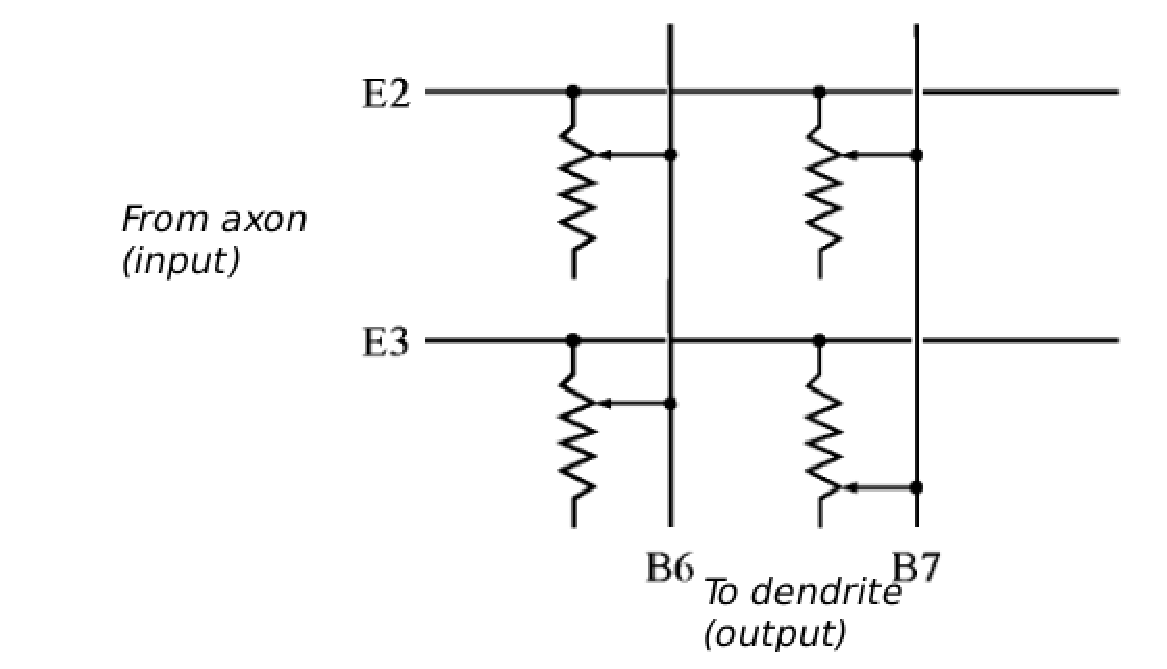
\includegraphics[height=5cm]{./images/Steinbuch_network.eps}}
  \caption{A small part of Steinbuch network}\label{fig:Steinbuch}
\end{figure}

The important part of such network is that it can store several sets
of correlations simultaneously, in a {\it superimposed manner}. In
this mode of memory storage, the individual item in memory is stored
distributively over many synapses, and each synapse participates in
storing many different items.


Later, Christopher Longuet-Higgins, Peter Buneman and David Willshaw
continued the studied of association in a network with the arrangement
of axons and dendrites similar to that of Steinbuch. For
simplification, assume that
\begin{itemize}
\item A synapse has only 2 states: on (active) and off (inactive) which
  correspond to 1 and 0, respectively.
\item States of synapse are independent of time.
\end{itemize}

In the below figure, Fig. \ref{fig:HBW_network}, each neuron is
connected by some other neurons. The status of connection is expressed
via $S_{ij}$ 
\begin{equation}\begin{split}
  S_{ij} &= 1 \text{   if there is a synapse between neuron i and j} \\
         &= 0 \text{   otherwise}
\end{split}
\end{equation}
\begin{figure}[htb]
  \centerline{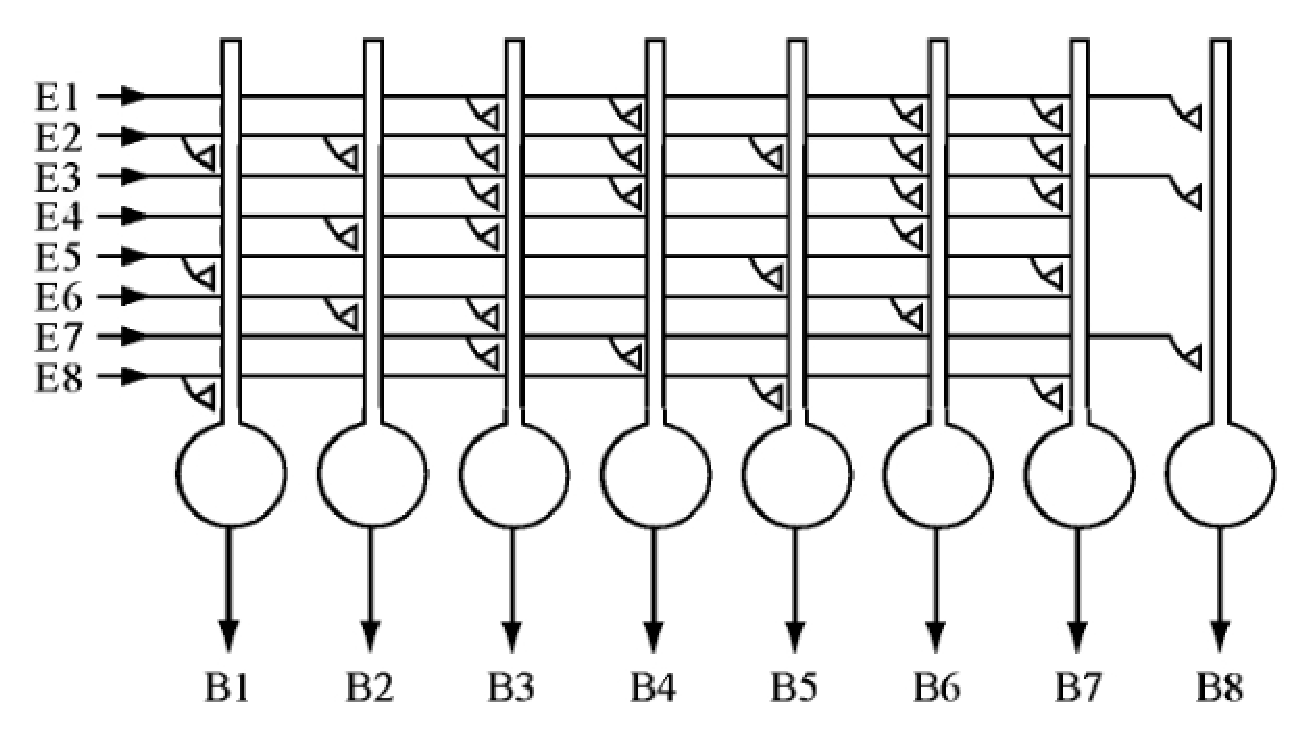
\includegraphics[height=5cm]{./images/HBW_network.eps}}
  \caption{Associate circuit of Higgins, Buneman and Willshaw network}\label{fig:HBW_network}
\end{figure}


Further, we denote $V_i$ the voltage at neuron $i$, at any
instant. Then, the voltage of a neuron depends upon the input stimuli
from other neurons via the formula
\begin{equation}
  V_i \rightarrow 1 \text{ if } \sum_{j\ne i} V_j S_{ij} \ge V_{threshold}
\end{equation}
end
\begin{equation}
  V_i \rightarrow 0 \text{ if } \sum_{j\ne i} V_j S_{ij} < V_{threshold}
\end{equation}

In the following example, we have only three of eight total neurons to be
active in any of the input pattern, so we set $V_{threshold} = 3$. 
\begin{itemize}
\item For the first input pattern: $V_i = {0 1 0 1 0 1 0 0
  }$. Accordingly, the output will be $B_j = {1 3 3 1 1 3 1 0}$. 
\item For the second input pattern: $V_i = {1 0 0 0 1 0 1 0
  }$. Accordingly, the output will be $B_j = {.............}$. 
\end{itemize}

If we relax the number of active neurons, then we will see some
deficiency of this model.
\begin{itemize}
\item For the first input pattern: $V_i = {1 1 1 1 1 1 1 1 
  }$. Accordingly, the output will be $B_j = {0 8 0 0 0 8 0 0}$ 
\item For the second input pattern: $V_i = {1 1 0 0 0 0 1 0 
  }$. Accordingly, the output will be $B_j = {0 5 0 0 0 5 0 0}$. 
\end{itemize}
Essentially, we get the same output for two different input
patterns. This may be trouble since the brain can not discriminate
things.The examined model invokes only binary responses. However, the
real neurons are capable of more graduated response. Further, the
given model always return alternative stable memories. There is no
status of all being faded away (i.e. dies away to zero or in
inhibitory state) as is frequently the case in neural network. Now, we
introduce another model that is closed to those encountered in
biology. 

{\bf Model 1:} Each neuron can be in either excitatory (white) or
inhibitory (black). It means that
{\it a given neuron can release only one type of neurotransmitter}
which falls into two classes: one that tend to depolarizes the
post-synaptic (excitatory) and one that tend to hyper-polarize the
post-synaptic (inhibitory). The role of inhibitory neurons is to
dampen down the activity level of excitatory group.  In this model, as
shown in Fig. \ref{fig:auto_assoc1}, inhibitory neurons (black) can
only receive stimuli from local neurons and it feed inhibition back to
these local neurons which activate them.
\begin{figure}[htb]
  \centerline{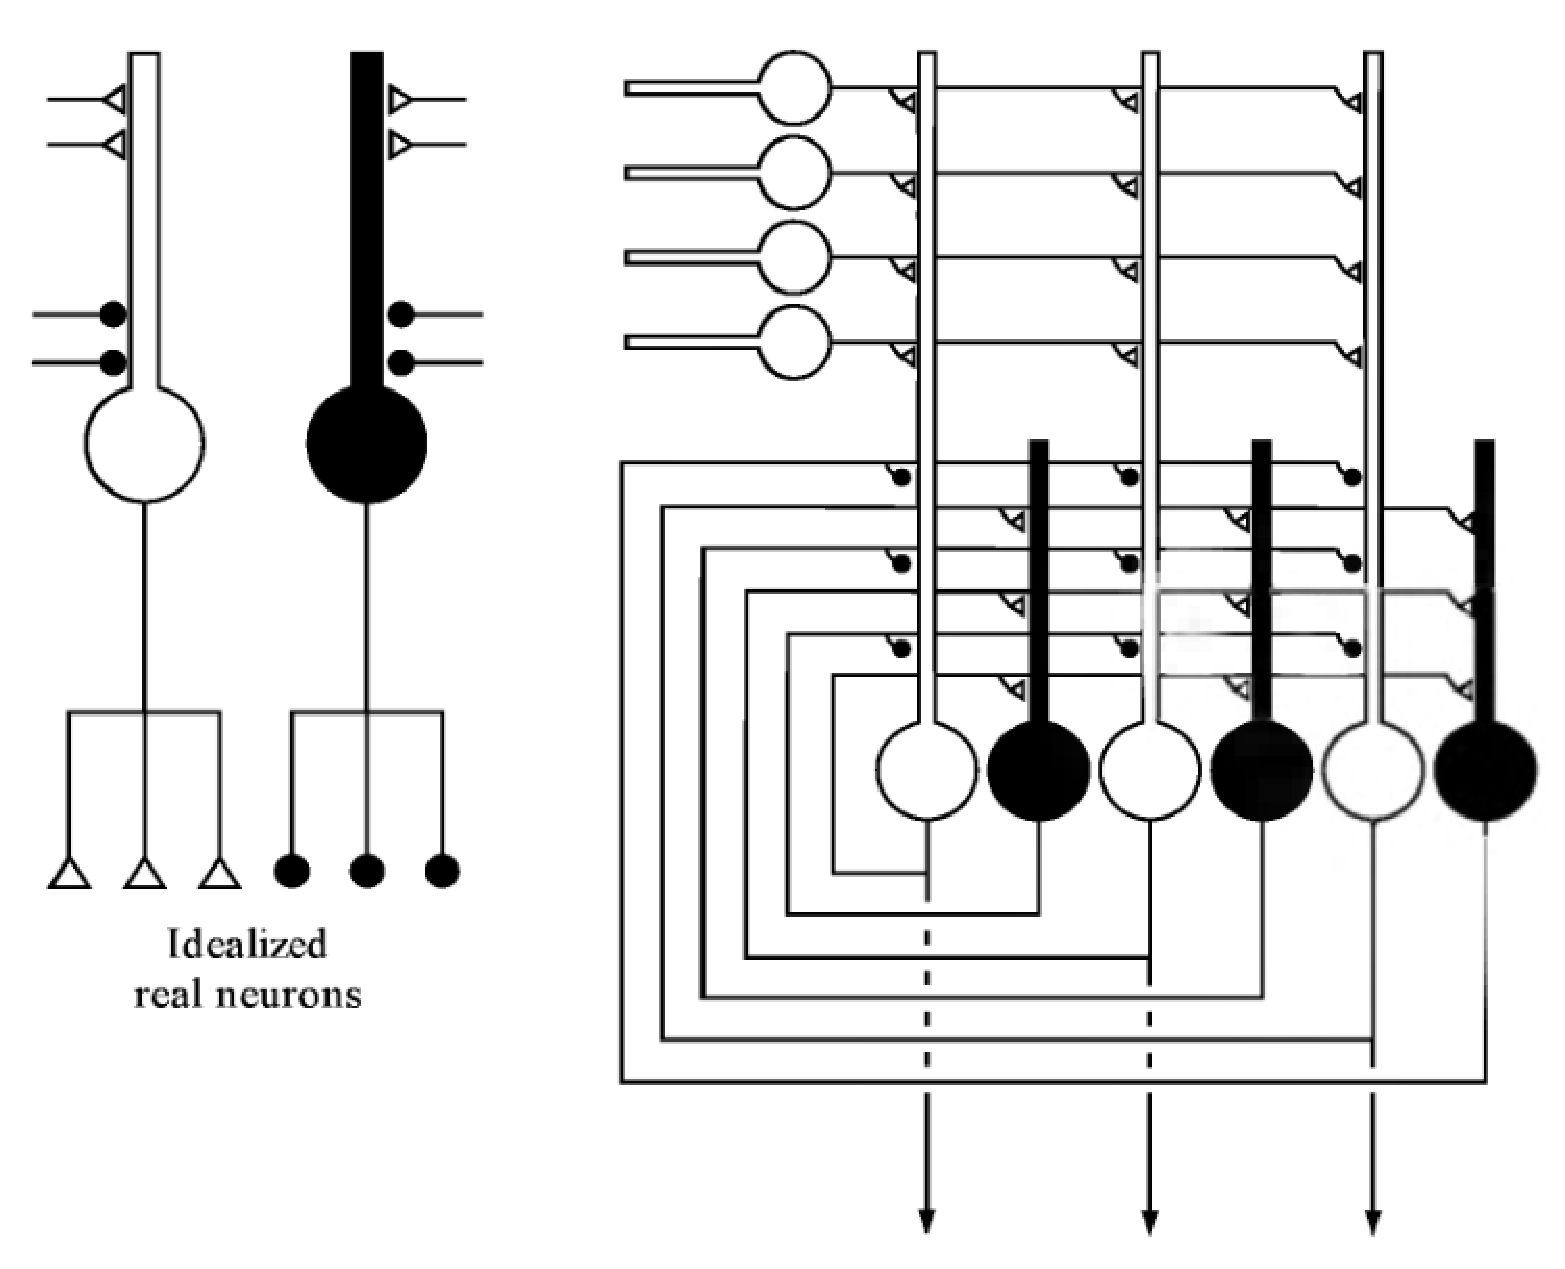
\includegraphics[height=6cm]{./images/inhibitory_excitatory_feedback.eps}}
  \caption{Inhibitory-excitatory model with feedback (white neuron:
    fire excitatory, black neuron: inhibitory}\label{fig:auto_assoc1}
\end{figure}



{\bf Model 2}: Another type of arrangement, in
Fig. \ref{fig:auto_assoc2}, is often found in brain, namely
{\it feed-forward inhibitory neurons}. The inhibitory neurons can
receives stimuli from neurons at greater distance and it feed
inhibition to other neurons (not to the ones that activate them).

\begin{figure}[htb]
  \centerline{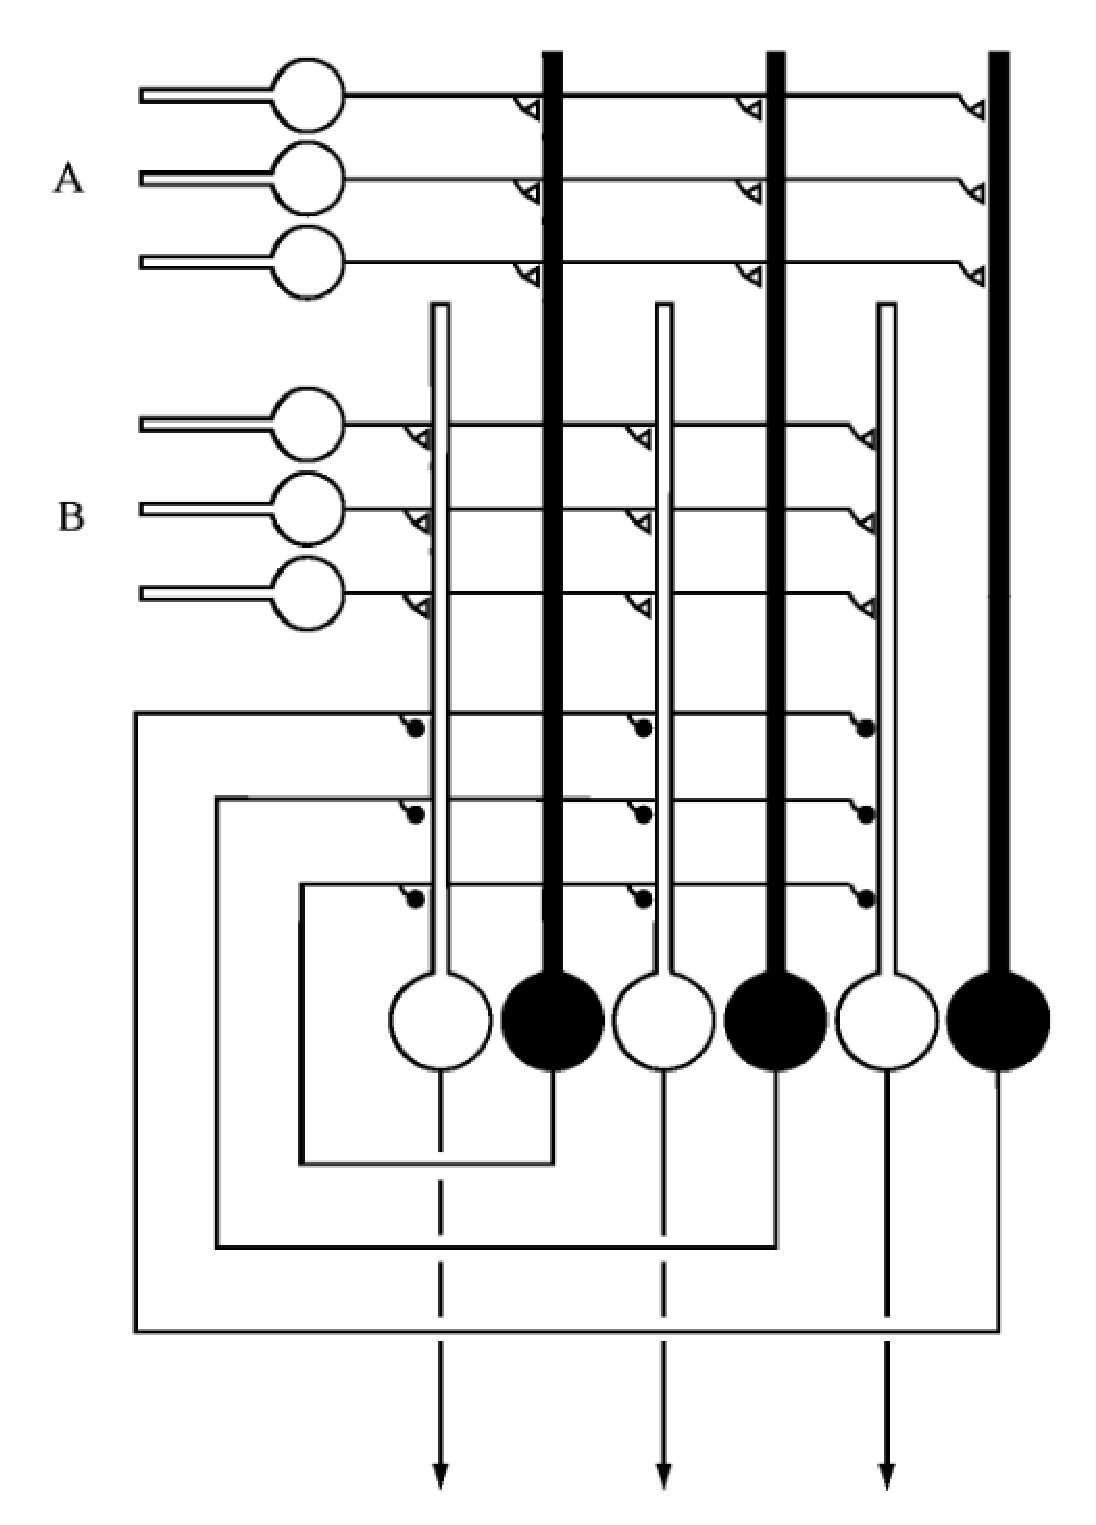
\includegraphics[height=6cm]{./images/inhibitory_excitatory_feedforward.eps}}
  \caption{Inhibitory-excitatory model with feedforward}\label{fig:auto_assoc2}
\end{figure}


IN SUMMARY:
\begin{itemize}
\item Distribution of synaptic strength demonstrates the correlation
  between inputs.
\item To store multiple memories, there should be multiple
  connections.
\item Memory is distributed.
\item A single synapse participates in many memory
\end{itemize}

\section{Self-organizing map (SOM)}
\label{sec:Self-organizing-map}


\section{Auto-associative network}

In the previous models, we haven't taken into account the function of
axon hillock, the inner part of the axon that is very close to the
soma. Structurally, the axon is frequently observed to branch into two
or more strands in which the main branch is still referred to as the
axon, while the subsidiary conduits are known as
{\it axon collaterals}. In the latter, there is an important sub-class
that arch back and form a synaptic contact with the dendrites  of the
same neuron. These are known as {\bf recurrent collaterals}.

By invoking such recurrent collaterals, Teuvo Kohonen demonstrated
that a group of neurons can {\it auto-associate}. In the following
figure, Fig. , the strength of the synapse is demonstrated by the
size of small triangles, which initially, being drawn at the same
size. 

\begin{figure}[htb]
  \centerline{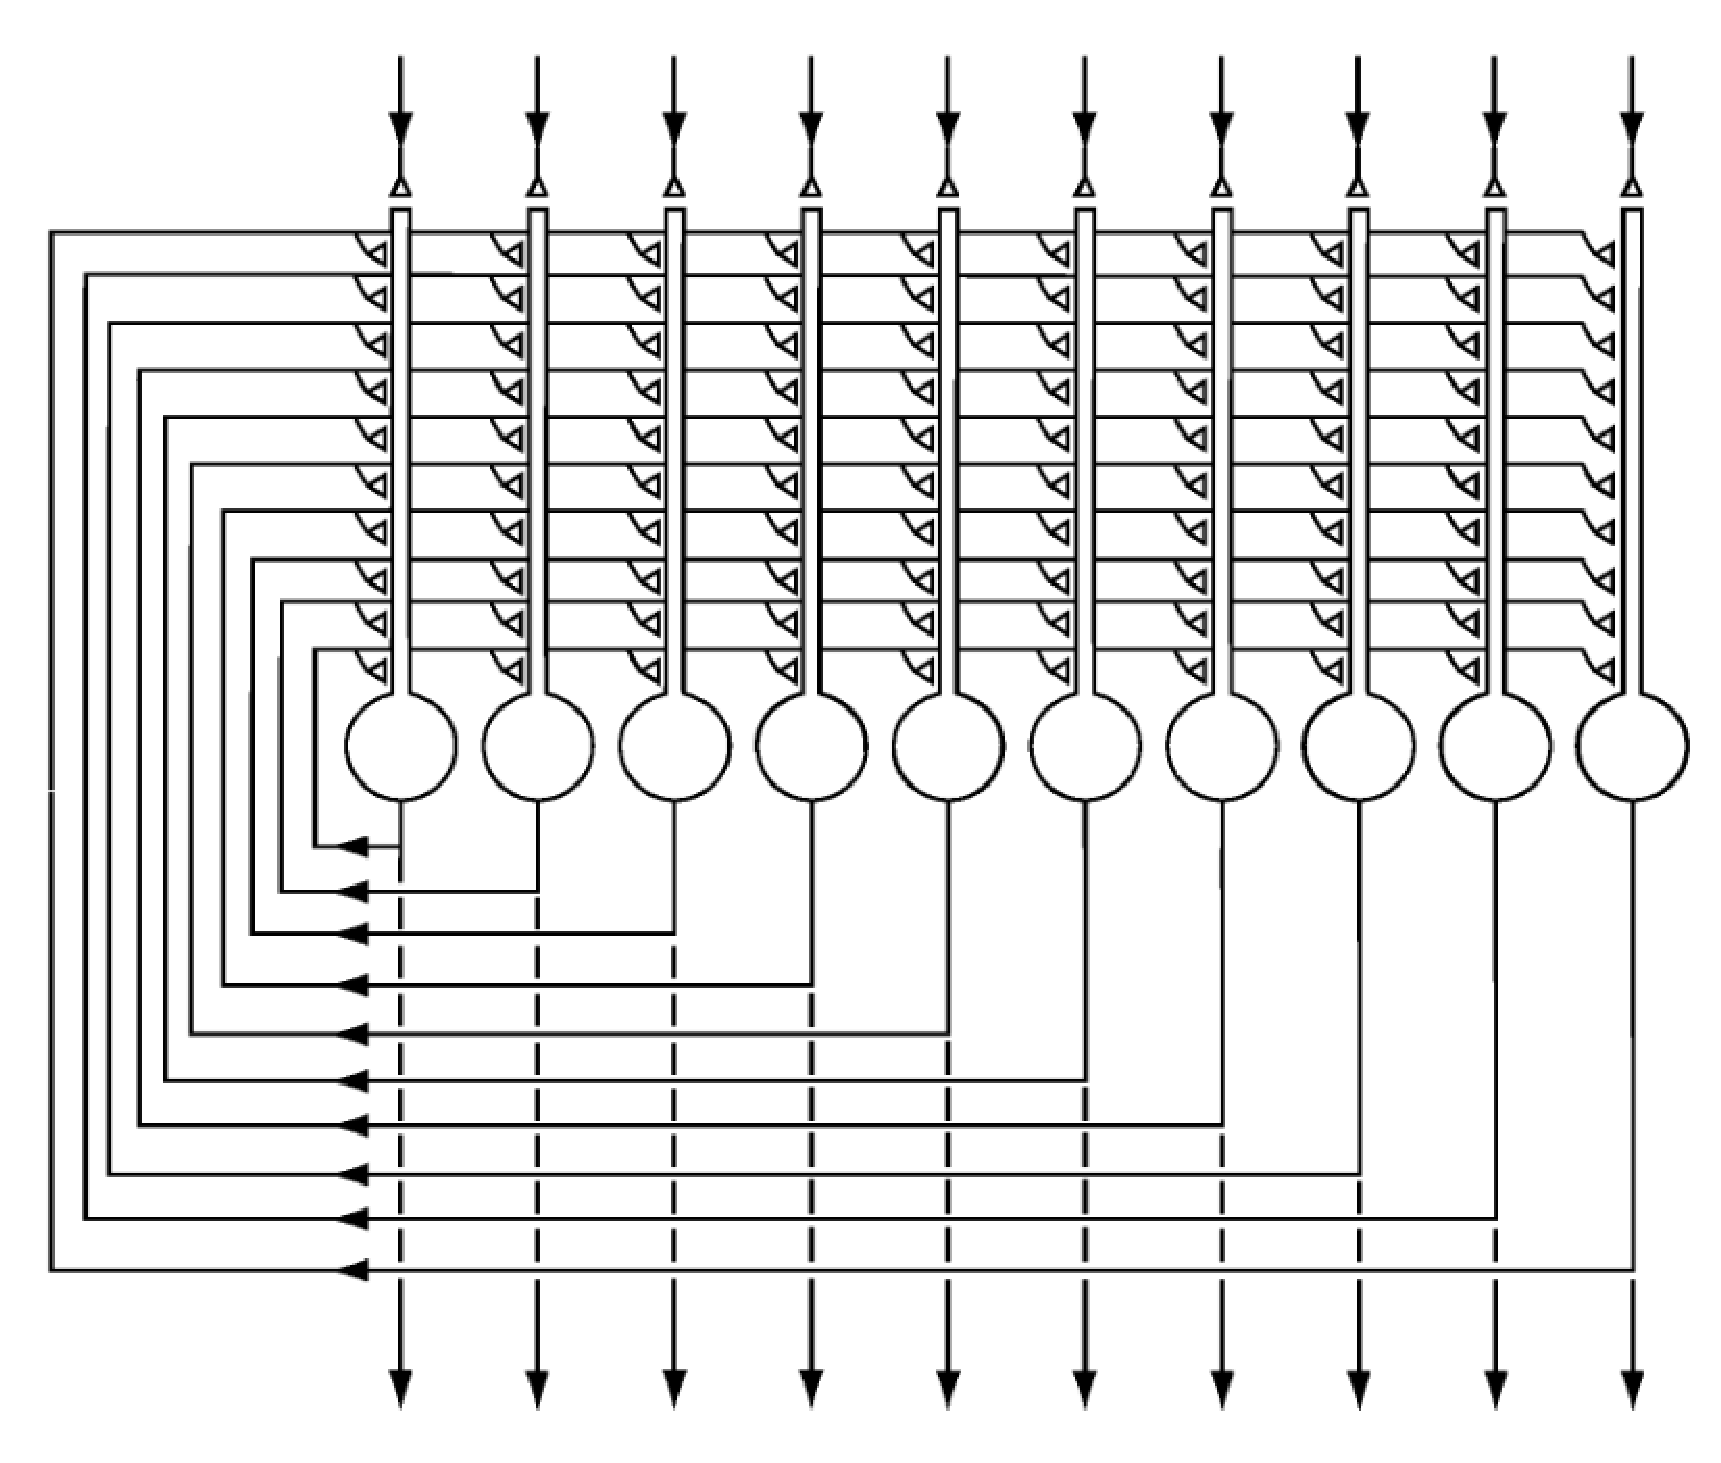
\includegraphics[height=5cm]{./images/auto_associative_network.eps}}
  \caption{Auto associative network}\label{fig:auto_assoc3}
\end{figure}
With this model, after training, it can generate the same output even
though there is a slightly change (or partial loss) in the input.

\begin{itemize}
\item At time $t = 0$: $V_{in(t=0)}$ a $n\times 1$ array
\item At time $t = \Delta t$: $V_{out(t=\Delta t)} = V_{in(t=0)}$ (a
  $n\times 1$ array) is the signal get out of the axon collaterals.
\item At time $t = 2\Delta t$: $V_{out(t=2\Delta t)} = \mathbf{S}.
  V_{out(t=\Delta t)}^*$ (a $n\times 1$ array) is the signal get out of
  the axon to be output pattern. {\bf S} is the matrix of connection.
\end{itemize}
where asterisk is a reminder that a component of a vector can exercise
an influence only if it is above the threshold.

This model of network, of course, has it memory capacity. If the
capacity has not been exceeded, it can superimpose the stored memories
upon one another; a given synapse participating in the recording of
all the memories and each memory being distributed all over the
synapses, as described in other previous models. However, this model
is robust against partial synaptic loss which is augmented by many
evidence that it's the same as the real brain process.


The {\bf dynamic link architecture} (DLA) hypothesis
has 2 central parts: (1) binding by signal
correlations, and (2) short-term synaptic modificatio
\url{http://willcov.com/bio-consciousness/sidebars/Dynamic Link Architecture.htm}




\section{Perforant pathway: EC to hippocampal formation}
\label{sec:perforant-pathway}

The {\bf perforant pathway} provides a connectional route from the entorhinal
cortex (EC, Sect.\ref{sec:entorhinal-cortex}), to all fields of the 
hippocampal formation (Sect.\ref{sec:hippocampal_formation}).

The pathway arises mainly from layer II and III of EC, yet it also
comprises a smaller component that originates in deep layers V and VI
\citep{witter2007}.

\begin{itemize}
  \item neurons in layer II (and possibly layer IV) project to the dentate gyrus
  (Sect.\ref{sec:dentate_gyrus}) and CA3 field
  
  \item neurons in layer III (and possibly layer V) project to CA1 field and
  subiculum via the temporoammonic pathway.
\end{itemize}


\section{dorsal/posterior column-medial lemniscus pathway (DCML, PCML)}
\label{sec:PCML}
\label{sec:DCML}

Posterior column-medial lemniscus pathway (PCML) (also known as the dorsal
column-medial lemniscus pathway) is a sensory pathway
(Sect.\ref{sec:somatosensory-pathways}) in the CNS that conveys the localized
sensation from the skins and joints via the ventroposterior medial nucleus
(VPM, Sect.\ref{sec:thalamus}), and finally to the postcentral gyrus
(Sect.\ref{sec:postcentral-gyrus}).

There are 3 neurons involved
\begin{enumerate}
  \item first-order neurons: (soma in the root ganglion) send input from
  skins/joins (via {\it cuneate fasciculus} (tract of Burdach, fasciculus cuneatus) - tract of
  nerves in spinal cords to transmit information from arms, and via
  {\it gracile fasciculus} (tract of Goll, fasciculus gracilis) - tract of
  axon fibers to carry the information from the lower limbs), 
  and then make
  contact with second-order neurons at at the gracile and cuneate nuclei in the lower medulla.
    
  \item second-order neurons: (soma in the brainstem) receive the input from
  first-order neurons, and send their axons to the third-order neurons in the thalamus.
  
  \item third-order neurons: send output to the postcentral gyrus.
\end{enumerate}

The PCML pathway is composed of rapidly conducting, large, myelinated fibers
{\tiny
\begin{verbatim}
 
   first-order   --->  second-order     ---> third-order  ---> postcentral gyrus
                  (cross medulla oblongata)    (in thalamus)
                                              travel to internal capsule
cuneate fascuculus |     
(lower body axons) 

gracile fasciculus |
(upper body axon)
\end{verbatim}
}
\url{https://en.wikipedia.org/wiki/Posterior_column-medial_lemniscus_pathway}

\section{Ventral spinothalamic pathways}
\label{sec:ventral-spinothalamic-pathway}

The ventral spinothalamic pathways cross the spinal cord.
There are two adjacent pathways
\begin{itemize}
    \item anterior ventral spinothalamic pathway: sense crude touch and
firm pressure 
    \item lateral ventral spinothalamic pathway: sense pain and
  temperature 
\end{itemize}

Like DCML (Sect.\ref{sec:DCML}), ether pathways use 3 layers of neurons:
\begin{enumerate}
  \item first-neurons: soma in the dorsal root ganglion, and the axon 
  lead to the dorsalspinal cord, and then synapse with the second-neurons.
  
  \item second-neurons: somas in the spinal cord, with axons
  synapse with the third-neurons at different nuclei in the thalamus 
(Sect.\ref{sec:thalamus}) 

% which also deals with information from other senses
% (vision + hearing), and passes the signals on to the {\bf somatosensory cortex}.
  
  \item third-neurons (touch or certain types of pain): the soma in
   the ventral posterior nuclei (VPN) of the thalamus, and project to
   the postcentral gyrus. 
\end{enumerate}
%The impulses travel along these nerve cells and reach the {\bf thalamus}

\section{*Dopaminergic pathways}
\label{sec:dopaminegic_pathways}

The dopaminergic pathways refers to the axon projection from dopaminergic
neurons (Sect.\ref{sec:dopaminegic_neurons}) in one region to the postsynaptic
neurons in another region.

\begin{figure}[hbt]
  \centerline{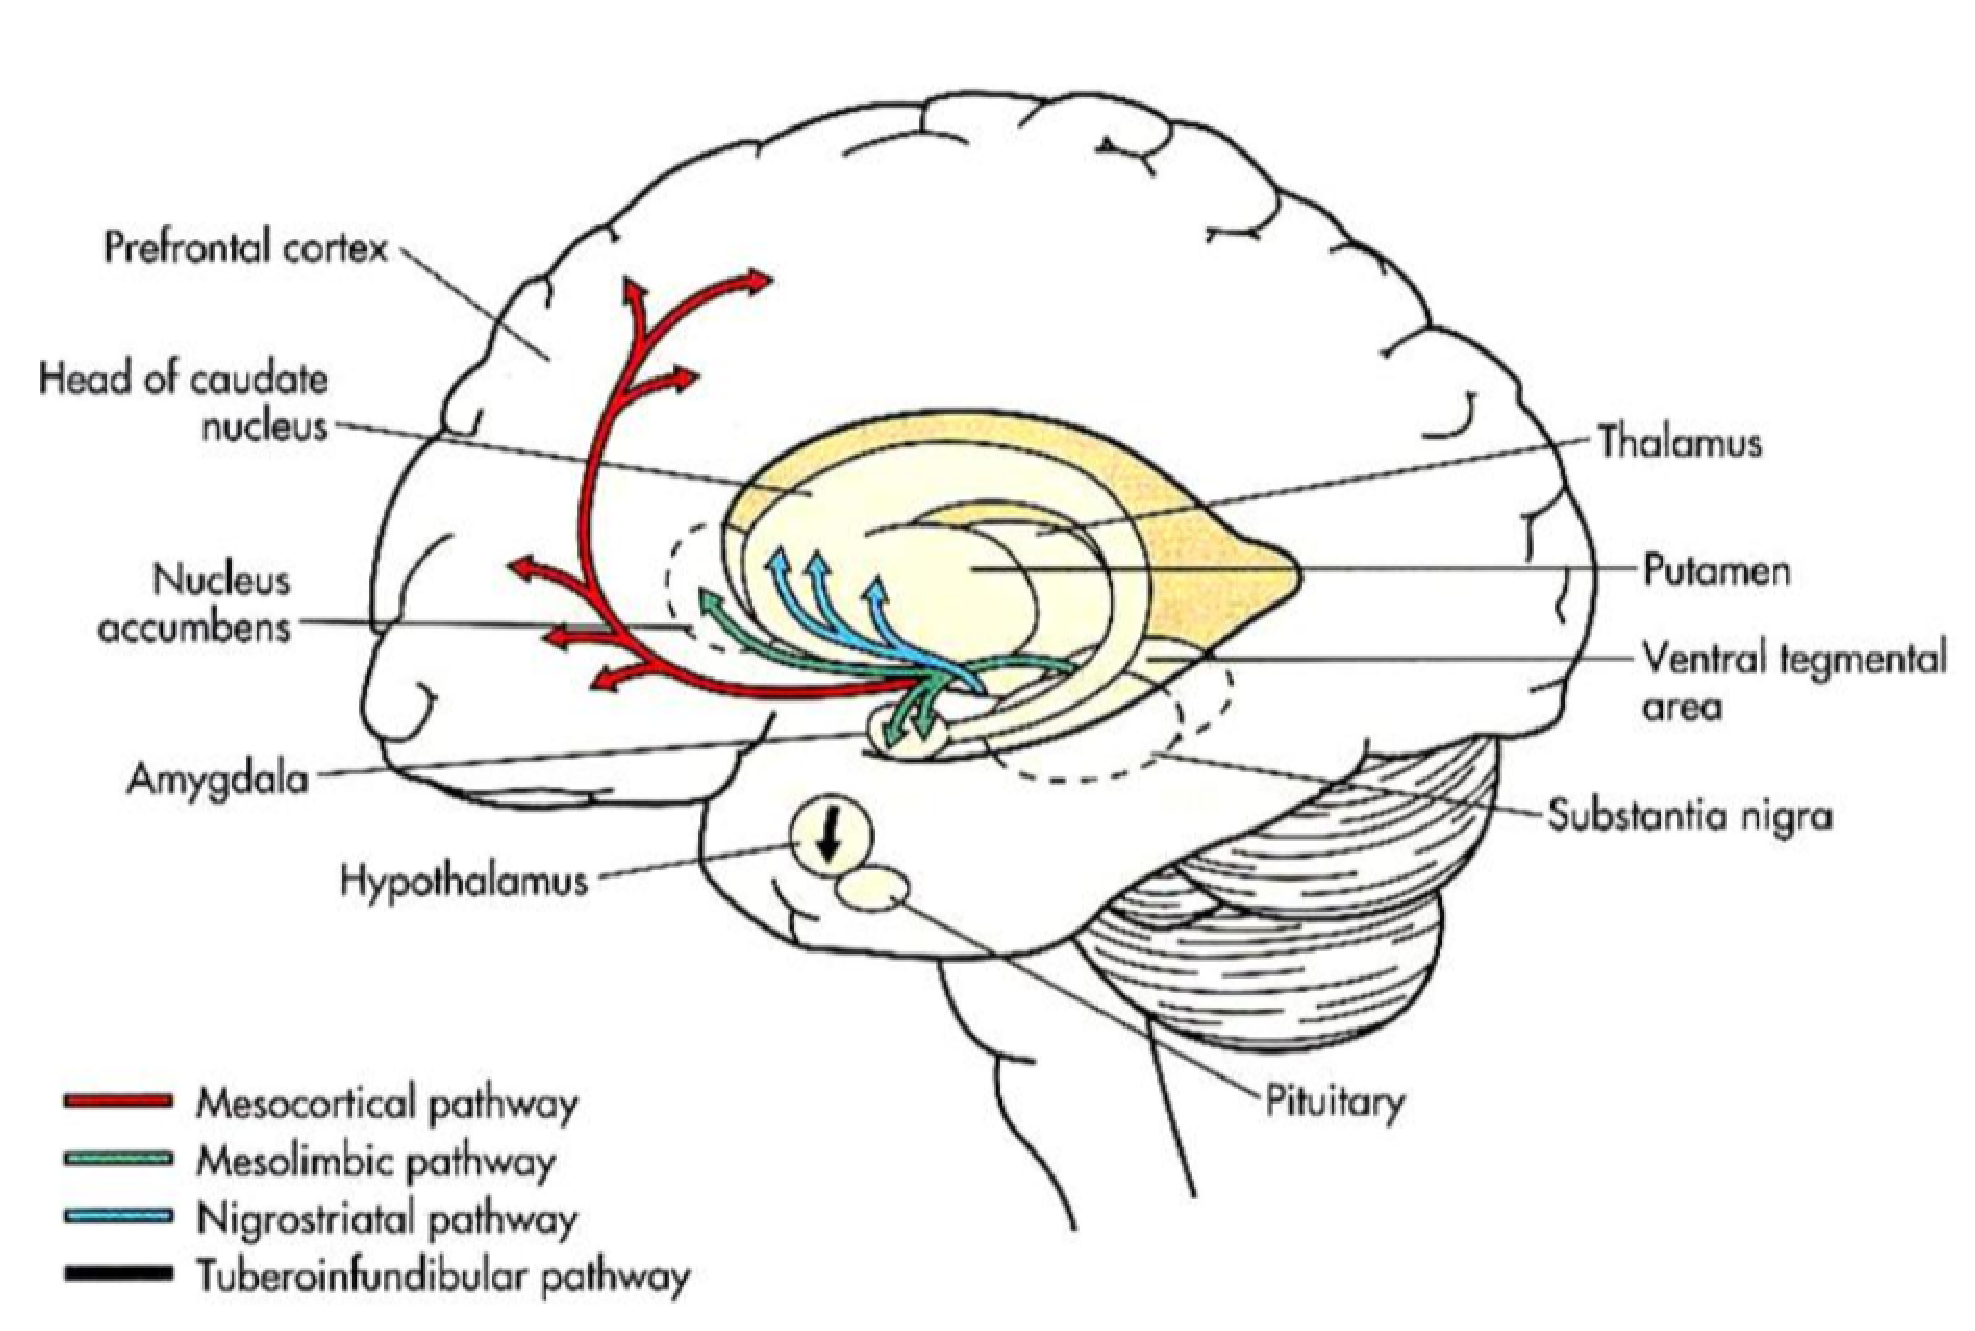
\includegraphics[height=6cm,
    angle=0]{./images/dopamine-pathways.eps}}
\caption{ERK }
\label{fig:dopaminergic-pathway}
\end{figure}


There are 8 pathways, but 4 major pathways, Fig.\ref{fig:dopaminergic-pathway}:
two major pathways are from VTA (Sect.\ref{sec:ventral-tegmented-area}) and one
major pathway is from substantia nigra pars compacta (Sect.\ref{sec:SNpc}), and
one major pathway is from hypothalamus in the limbic system
(Sect.\ref{sec:hypothalamus}).
(review: \citep{beaulieu2011})

% ; the nigrostriatal, mesolimbic,
% mesocortical and tuberoinfundibular systems that originate from the A9 (nigrostriatal), A10 (mesolimbic and mesocortical, often
% collectively termed the mesocorticolimbic pathway), and A8 (tuberoinfundibular)
% groups of dopamine-containing cell 

\textcolor{red}{4 major dopaminergic pathways}
\begin{enumerate}
  \item mesolimbic pathway (Sect.\ref{sec:mesolimbic-pathway}): originate from
  A10 cells

  \item mesocortical pathway (Sect.\ref{sec:mesocortical-pathway})
  
  \item nigrostriatal pathway (Sect.\ref{sec:nigrostriatal-pathway}): originate
  from A9 cells
  
  
  \item tuberoinfundibular pathway - Sect.\ref{sec:tuberoinfundibular-pathway}:
  originate from A8 cells
\end{enumerate}

\textcolor{red}{4 minor dopaminergic pathways}: These are the 4 pathways found
in VTA (Sect.\ref{sec:ventral-tegmented-area})
\begin{enumerate}
  \item VTA $\rightarrow$ Amygdala (Sect.\ref{sec:amygdala})
  
  \item VTA $\rightarrow$ Cingulate gyrus (Sect.\ref{sec:cingulate_gyrus})
  
  \item VTA $\rightarrow$ Hippocampus (Sect.\ref{sec:hippocampus})
  
  \item VTA $\rightarrow$ Olfactory bulb (Sect.\ref{sec:olfactory-bulb})
 
\end{enumerate}

\section{- Mesolimbic pathway (reward pathway)}
\label{sec:mesolimbic-pathway}

The mesolimbic pathway, sometimes referred to as the reward pathway, is a
dopaminergic pathway (Sect.\ref{sec:dopaminegic_pathways}) connecting VTA
(Sect.\ref{sec:ventral-tegmented-area}) to nucleus accumbens (NAc) via medial
forebrain bundle (a tract containing fibers) - Sect.\ref{sec:nucleus_accumbens}.



It is: VTA $\rightarrow$ nucleus accumbens.
  

\section{- Mesocortical pathway}
\label{sec:mesocortical-pathway}

Mesocortical pathway is a dopaminegic pathway
(Sect.\ref{sec:dopaminegic_pathways}) connecting VTA
(Sect.\ref{sec:ventral-tegmented-area}) to the prefrontal cortex
(Sect.\ref{sec:prefrontal-cortex}).

It is: VTA $\rightarrow$ prefrontal cortex.




\section{- Nigrostriatal pathway}
\label{sec:nigrostriatal-pathway}

The {\bf nigrostriatal pathway} is a dopaminergic pathway
(Sect.\ref{sec:dopaminegic_pathways}) connecting SNpc (Sect.\ref{sec:SNpc}) to
the D1-MSN in (dorsal) striatum (Sect.\ref{sec:D1-MSN}).

% The nigrostriatal projection has two terminal fields:
% \begin{itemize}
%   \item (major projection) striatum: caudate and putamen
%   
%   \item (most posterior dopaminergic neurons's projection)
% \end{itemize}

IMPORTANT: Dopamine releasing neurons of this pathway release several other
neurotransmitters, including glutamate \citep{tecuapetla2010} and GABA
\citep{tritsch2012}.




\section{- Tuberoinfundibular pathway}
\label{sec:tuberoinfundibular-pathway}

